\def\paperversiondraft{draft}
\def\paperversionnormal{normal}

% If the paper version is set to 'normal' mode keep it,
% otherwise set it to 'draft' mode.
\ifx\paperversion\paperversionnormal
\else
  \def\paperversion{draft}
\fi

\documentclass[review, anonymous, sigplan]{acmart}

\def\acmversionanonymous{anonymous}
\def\acmversionjournal{journal}
\def\acmversionnone{none}

\makeatletter
\if@ACM@anonymous
  \def\acmversion{anonymous}
\else
  \def\acmversion{journal}
\fi
\makeatother

\usepackage{colortbl}

% 'draftonly' environment
\usepackage{environ}
\ifx\paperversion\paperversiondraft
\newenvironment{draftonly}{}{}
\else
\NewEnviron{draftonly}{}
\fi

% Most PL conferences are edited by conference-publishing.com. Follow their
% advice to add the following packages.
%
% The first enables the use of UTF-8 as character encoding, which is the
% standard nowadays. The second ensures the use of font encodings that support
% accented characters etc. (Why should I use this?). The mictotype package
% enables certain features 'to­wards ty­po­graph­i­cal per­fec­tion
\usepackage[utf8]{inputenc}
\usepackage[T1]{fontenc}
\usepackage{microtype}

\usepackage{xargs}
\usepackage{lipsum}
\usepackage{xparse}
\usepackage{xifthen, xstring}
\usepackage{xspace}
\usepackage{marginnote}
\usepackage{etoolbox}
\usepackage[acronym,shortcuts]{glossaries}
\usepackage{amsmath}
\usepackage{thmtools} % required for autoref to lemmas
\usepackage{algorithm}
\usepackage[noend]{algpseudocode}
\usepackage{xfp}
\usepackage{hyphenat}
\usepackage[shortcuts]{extdash}

%%%%%%%%%%%%%%%%%%%%%%%%%%%%%%%%%%%%%%%%%%%%%%%%%%%%%%%%%%%%%%%%%%%%%%%%%%%%%%%
% Broaden margins to make room for todo notes
%%%%%%%%%%%%%%%%%%%%%%%%%%%%%%%%%%%%%%%%%%%%%%%%%%%%%%%%%%%%%%%%%%%%%%%%%%%%%%%

\makeatletter
\patchcmd{\@addmarginpar}{\ifodd\c@page}{\ifodd\c@page\@tempcnta\m@ne}{}{}
\makeatother
\ifx\paperversion\paperversiondraft
  \makeatletter
  \if@ACM@journal
    \geometry{asymmetric}
    \paperwidth=\dimexpr \paperwidth + 3.5cm\relax
    \oddsidemargin=\dimexpr\oddsidemargin + 0cm\relax
    \evensidemargin=\dimexpr\evensidemargin + 0cm\relax
    \marginparwidth=\dimexpr \marginparwidth + 3cm\relax
    \setlength{\marginparwidth}{4.6cm}
    % This makeatletter box helps to move notes to the right
    \makeatletter
    \long\def\@mn@@@marginnote[#1]#2[#3]{%
      \begingroup
        \ifmmode\mn@strut\let\@tempa\mn@vadjust\else
          \if@inlabel\leavevmode\fi
          \ifhmode\mn@strut\let\@tempa\mn@vadjust\else\let\@tempa\mn@vlap\fi
        \fi
        \@tempa{%
          \vbox to\z@{%
            \vss
            \@mn@margintest
            \if@reversemargin\if@tempswa
                \@tempswafalse
              \else
                \@tempswatrue
            \fi\fi
            %\if@tempswa
              \rlap{%
                \if@mn@verbose
                  \PackageInfo{marginnote}{xpos seems to be \@mn@currxpos}%
                \fi
                \begingroup
                  \ifx\@mn@currxpos\relax\else\ifx\@mn@currxpos\@empty\else
                      \kern-\dimexpr\@mn@currxpos\relax
                  \fi\fi
                  \ifx\@mn@currpage\relax
                    \let\@mn@currpage\@ne
                  \fi
                  \if@twoside\ifodd\@mn@currpage\relax
                      \kern\oddsidemargin
                    \else
                      \kern\evensidemargin
                    \fi
                  \else
                    \kern\oddsidemargin
                  \fi
                  \kern 1in
                \endgroup
                \kern\marginnotetextwidth\kern\marginparsep
                \vbox to\z@{\kern\marginnotevadjust\kern #3
                  \vbox to\z@{%
                    \hsize\marginparwidth
                    \linewidth\hsize
                    \kern-\parskip
                    \marginfont\raggedrightmarginnote\strut\hspace{\z@}%
                    \ignorespaces#2\endgraf
                    \vss}%
                  \vss}%
              }%
          }%
        }%
      \endgroup
    }
    \makeatother
  \else
    \paperwidth=\dimexpr \paperwidth + 6cm\relax
    \oddsidemargin=\dimexpr\oddsidemargin + 3cm\relax
    \evensidemargin=\dimexpr\evensidemargin + 3cm\relax
    \marginparwidth=\dimexpr \marginparwidth + 3cm\relax
    \setlength{\marginparwidth}{4.6cm}
  \fi
  \makeatother
\fi

%%%%%%%%%%%%%%%%%%%%%%%%%%%%%%%%%%%%%%%%%%%%%%%%%%%%%%%%%%%%%%%%%%%%%%%%%%%%%%%
% Add \createtodoauthor command
%%%%%%%%%%%%%%%%%%%%%%%%%%%%%%%%%%%%%%%%%%%%%%%%%%%%%%%%%%%%%%%%%%%%%%%%%%%%%%%

\usepackage[textsize=tiny]{todonotes}
\usepackage[normalem]{ulem}

\makeatletter
\font\uwavefont=lasyb10 scaled 652
\newcommand\colorwave[1][blue]{\bgroup\markoverwith{\lower3\p@\hbox{\uwavefont\textcolor{#1}{\char58}}}\ULon}

\newcommand\highlight[2]{{\color{#1}{\colorwave[#1]{#2}}}}
\makeatother

\makeatletter
\newcommand\InFloat[2]{\ifnum\@floatpenalty<0\relax#1\else#2\fi}
\makeatother

\newboolean{inComment}
\setboolean{inComment}{false}

\ifx\paperversion\paperversiondraft
\newcommand\createtodoauthor[2]{
  \def\tmpdefault{emptystring}
  \expandafter\newcommand\csname #1\endcsname[2][\tmpdefault]{% comment to avoid spurious whitespace
    \ifthenelse{\boolean{inComment}}{% comment to avoid spurious whitespace
      \PackageError{paper-template}{Comments in comments not supported}{}% comment to avoid spurious whitespace
    }{}\setboolean{inComment}{true}% comment to avoid spurious whitespace
    \def\tmp{##1}% comment to avoid spurious whitespace
    \InFloat{
        \smash{
	  \marginnote{
	    \todo[inline,linecolor=#2,backgroundcolor=#2,bordercolor=#2]
	      {\textbf{#1 (Figure):} ##2}
          }
        }
    }{\ifthenelse{\equal{\tmp}{\tmpdefault}} % Is there text to highlight?
      {\todo[linecolor=#2,backgroundcolor=#2,bordercolor=#2]{\textbf{#1:} ##2}\ignorespaces}
      {\ifthenelse{\equal{##2}{}} % Is there a note?
        {\highlight{#2}{##1}}
        {\highlight{#2}{##1}\todo[linecolor=#2,backgroundcolor=#2,bordercolor=#2]
	  {\textbf{#1:} ##2}% comment to avoid spurious whitespace
	}% comment to avoid spurious whitespace
      }% comment to avoid spurious whitespace
    }% comment to avoid spurious whitespace
    \setboolean{inComment}{false}% comment to avoid spurious whitespace
  }
}
\else
\newcommand\createtodoauthor[2]{%
\expandafter\newcommand\csname #1\endcsname[2][]{##1}%
}%
\fi

%%%%%%%%%%%%%%%%%%%%%%%%%%%%%%%%%%%%%%%%%%%%%%%%%%%%%%%%%%%%%%%%%%%%%%%%%%%%%%%
% Add minted and support custom lexers
%%%%%%%%%%%%%%%%%%%%%%%%%%%%%%%%%%%%%%%%%%%%%%%%%%%%%%%%%%%%%%%%%%%%%%%%%%%%%%%
\usepackage{minted}
\usepackage{etoolbox}

\makeatletter
\ifcsdef{minted@optlistcl@quote}
{
\ifwindows
  \renewcommand{\minted@optlistcl@quote}[2]{%
    \ifstrempty{#2}{\detokenize{#1}}{\detokenize{#1="#2"}}}
\else
  \renewcommand{\minted@optlistcl@quote}[2]{%
    \ifstrempty{#2}{\detokenize{#1}}{\detokenize{#1='#2'}}}
\fi

% similar to \minted@def@optcl@switch
\newcommand{\minted@def@optcl@novalue}[2]{%
  \define@booleankey{minted@opt@g}{#1}%
    {\minted@addto@optlistcl{\minted@optlistcl@g}{#2}{}%
     \@namedef{minted@opt@g:#1}{true}}
    {\@namedef{minted@opt@g:#1}{false}}
  \define@booleankey{minted@opt@g@i}{#1}%
    {\minted@addto@optlistcl{\minted@optlistcl@g@i}{#2}{}%
     \@namedef{minted@opt@g@i:#1}{true}}
    {\@namedef{minted@opt@g@i:#1}{false}}
  \define@booleankey{minted@opt@lang}{#1}%
    {\minted@addto@optlistcl@lang{minted@optlistcl@lang\minted@lang}{#2}{}%
     \@namedef{minted@opt@lang\minted@lang:#1}{true}}
    {\@namedef{minted@opt@lang\minted@lang:#1}{false}}
  \define@booleankey{minted@opt@lang@i}{#1}%
    {\minted@addto@optlistcl@lang{minted@optlistcl@lang\minted@lang @i}{#2}{}%
     \@namedef{minted@opt@lang\minted@lang @i:#1}{true}}
    {\@namedef{minted@opt@lang\minted@lang @i:#1}{false}}
  \define@booleankey{minted@opt@cmd}{#1}%
      {\minted@addto@optlistcl{\minted@optlistcl@cmd}{#2}{}%
        \@namedef{minted@opt@cmd:#1}{true}}
      {\@namedef{minted@opt@cmd:#1}{false}}
}
\minted@def@optcl@novalue{customlexer}{-x}
}
{
}
\makeatother

\usepackage{tikz}
\usetikzlibrary{arrows}
\usetikzlibrary{shapes}

%%%%%%%%%%%%%%%%%%%%%%%%%%%%%%%%%%%%%%%%%%%%%%%%%%%%%%%%%%%%%%%%%%%%%%%%%%%%%%%
% Base style and command for \circled to print a colored circle
%%%%%%%%%%%%%%%%%%%%%%%%%%%%%%%%%%%%%%%%%%%%%%%%%%%%%%%%%%%%%%%%%%%%%%%%%%%%%%%
% Width is assured to be the same across all characters using the typewriter font which is monospaced
% Zeroing out the inner separator removes padding between content and node (inner sep).
% Zeroing out the outer separator removes space between the node border and its anchors (e.g., east).
% Minimum size was derived on experimentation and it may need adjustment when changing font style/size.
%
% There is no guarantee for the letter ascenders/descenders to baseline when set to char.base, hence adding \strut.
% which is an invisible vertical rule with the height and depth of the parentheses ( and ).
% It ensures that the line height in a line of text is at least as large as if it contained parentheses. 
\tikzset{
  circledstyle/.style={
    shape=circle,
    #1,
    font=\tt\small,
    inner sep=0pt,
    outer sep=0pt,
    minimum size=1.2em,
    text=black
  }
}

% define a base tikz node for circled commands accepting a fill colour and the node text as arguments
\DeclareRobustCommand{\circledbase}[3][]{%
    \tikz[baseline=(char.base)]{\node[circledstyle, fill=#2] (char) {#3\strut};}%
}

%%%%%%%%%%%%%%%%%%%%%%%%%%%%%%%%%%%%%%%%%%%%%%%%%%%%%%%%%%%%%%%%%%%%%%%%%%%%%%%
% Add refcheck support
%%%%%%%%%%%%%%%%%%%%%%%%%%%%%%%%%%%%%%%%%%%%%%%%%%%%%%%%%%%%%%%%%%%%%%%%%%%%%%%
\usepackage[norefs,nocites]{refcheck}

% make refcheck work with autoref
% based on: https://tex.stackexchange.com/questions/87610/making-refcheck-work-with-cleveref
\makeatletter
\newcommand{\refcheckize}[1]{%
  \expandafter\let\csname @@\string#1\endcsname#1%
  \expandafter\DeclareRobustCommand\csname relax\string#1\endcsname[1]{%
    \csname @@\string#1\endcsname{##1}\wrtusdrf{##1}}%
  \expandafter\let\expandafter#1\csname relax\string#1\endcsname
}
\makeatother

%%% add the reference commands we want refcheck to be aware of
\refcheckize{\autoref}


\ifx\acmversion\acmversionjournal
  %% Journal information (used by PACMPL format)
  %% Supplied to authors by publisher for camera-ready submission
  \acmJournal{PACMPL}
  \acmVolume{1}
  \acmNumber{1}
  \acmArticle{1}
  \acmYear{2017}
  \acmMonth{1}
  \acmDOI{10.1145/nnnnnnn.nnnnnnn}
  \startPage{1}
\else
  %% Conference information (used by SIGPLAN proceedings format)
  %% Supplied to authors by publisher for camera-ready submission
  \acmConference[PL'17]{ACM SIGPLAN Conference on Programming Languages}{January 01--03, 2017}{New York, NY, USA}
  \acmYear{2017}
  \acmISBN{978-x-xxxx-xxxx-x/YY/MM}
  \acmDOI{10.1145/nnnnnnn.nnnnnnn}
  \startPage{1}
\fi

%% Copyright information
%% Supplied to authors (based on authors' rights management selection;
%% see authors.acm.org) by publisher for camera-ready submission
%\setcopyright{none}             %% For review submission
%\setcopyright{acmcopyright}
%\setcopyright{acmlicensed}
%\setcopyright{rightsretained}
%\copyrightyear{2017}           %% If different from \acmYear


%% Bibliography style
\bibliographystyle{ACM-Reference-Format}
%% Citation style
%% Note: author/year citations are required for papers published as an
%% issue of PACMPL.
%\citestyle{acmauthoryear}  %% For author/year citations
%\citestyle{acmnumeric}     %% For numeric citations
%\setcitestyle{nosort}      %% With 'acmnumeric', to disable automatic
                            %% sorting of references within a single citation;
                            %% e.g., \cite{Smith99,Carpenter05,Baker12}
                            %% rendered as [14,5,2] rather than [2,5,14].
%\setcitesyle{nocompress}   %% With 'acmnumeric', to disable automatic
                            %% compression of sequential references within a
                            %% single citation;
                            %% e.g., \cite{Baker12,Baker14,Baker16}
                            %% rendered as [2,3,4] rather than [2-4].


\usemintedstyle{colorful}

% Newer versions of minted require the 'customlexer' argument for custom lexers
% whereas older versions require the '-x' to be passed via the command line.
\makeatletter
\ifcsdef{MintedExecutable}
{
  % minted v3
  \newminted[mlir]{tools/lexers/MLIRLexer.py:MLIRLexerOnlyOps}{mathescape}
  \newminted[xdsl]{tools/lexers/MLIRLexer.py:MLIRLexer}{mathescape, style=murphy}
  \newminted[lean4]{tools/lexers/Lean4Lexer.py:Lean4Lexer}{mathescape}
}
{
  \ifcsdef{minted@optlistcl@quote}
  {
    \newminted[mlir]{tools/lexers/MLIRLexer.py:MLIRLexerOnlyOps}{customlexer, mathescape}
    \newminted[xdsl]{tools/lexers/MLIRLexer.py:MLIRLexer}{customlexer, mathescape, style=murphy}
    \newminted[lean4]{tools/lexers/Lean4Lexer.py:Lean4Lexer}{customlexer, mathescape}
  }
  {
    \newminted[mlir]{tools/lexers/MLIRLexer.py:MLIRLexerOnlyOps -x}{mathescape}
    \newminted[xdsl]{tools/lexers/MLIRLexer.py:MLIRLexer -x}{mathescape, style=murphy}
    \newminted[lean4]{tools/lexers/Lean4Lexer.py:Lean4Lexer -x}{mathescape}
  }
}
\makeatother

% We use the following color scheme
% 
% This scheme is both print-friendly and colorblind safe for
% up to four colors (including the red tones makes it not
% colorblind safe any more)
%
% https://colorbrewer2.org/#type=qualitative&scheme=Paired&n=4

\definecolor{pairedNegOneLightGray}{HTML}{cacaca}
\definecolor{pairedNegTwoDarkGray}{HTML}{827b7b}
\definecolor{pairedOneLightBlue}{HTML}{a6cee3}
\definecolor{pairedTwoDarkBlue}{HTML}{1f78b4}
\definecolor{pairedThreeLightGreen}{HTML}{b2df8a}
\definecolor{pairedFourDarkGreen}{HTML}{33a02c}
\definecolor{pairedFiveLightRed}{HTML}{fb9a99}
\definecolor{pairedSixDarkRed}{HTML}{e31a1c}

\createtodoauthor{grosser}{pairedOneLightBlue}
\createtodoauthor{authorTwo}{pairedTwoDarkBlue}
\createtodoauthor{authorThree}{pairedThreeLightGreen}
\createtodoauthor{authorFour}{pairedFourDarkGreen}
\createtodoauthor{authorFive}{pairedFiveLightRed}
\createtodoauthor{authorSix}{pairedSixDarkRed}

\newacronym{ir}{IR}{Intermediate Representation}

\graphicspath{{./images/}}

% Define macros that are used in this paper
%
% We require all macros to end with a delimiter (by default {}) to enusure
% that LaTeX adds whitespace correctly.
\makeatletter
\newcommand\requiredelimiter[2][########]{%
  \ifdefined#2%
    \def\@temp{\def#2#1}%
    \expandafter\@temp\expandafter{#2}%
  \else
    \@latex@error{\noexpand#2undefined}\@ehc
  \fi
}
\@onlypreamble\requiredelimiter
\makeatother

\newcommand\newdelimitedcommand[2]{
\expandafter\newcommand\csname #1\endcsname{#2}
\expandafter\requiredelimiter
\csname #1 \endcsname
}

\newdelimitedcommand{toolname}{Tool}

% helper macro to fully expand dimension expressions
\newcommand{\expanddim}[1]{\the\dimexpr#1\relax}

% Define the conversion function from any length to inches
\makeatletter
\newcommand{\convertToInches}[2]{%
  \edef\@temp{\expandafter\expandafter\expandafter\strip@pt\expandafter\dimexpr#1\relax}%
  \edef#2{\fpeval{round(\@temp / 72.27, 2)}}%
}
\makeatother

% create a new file for output
\newwrite\myfile
\immediate\openout\myfile=\jobname-layout.csv

% write widths to file
\makeatletter
\newcommand{\writePageWidths}{
  \newcommand{\mylen}{}%
  \convertToInches{\columnwidth}{\mylen}%
  \immediate\write\myfile{columnwidth, \mylen}%
  \convertToInches{\textwidth}{\mylen}%
  \immediate\write\myfile{textwidth, \mylen}%
  \convertToInches{\columnsep}{\mylen}%
  \immediate\write\myfile{columnsep, \mylen}%
  \convertToInches{\textheight}{\mylen}%
  \immediate\write\myfile{textheight, \mylen}%
  \convertToInches{\paperwidth}{\mylen}%
  \immediate\write\myfile{paperwidth, \mylen}%
  \convertToInches{\paperheight}{\mylen}%
  \immediate\write\myfile{paperheight, \mylen}%
}
\makeatother

\AtEndDocument{
  \writePageWidths
}

\usepackage{booktabs}
\newcommand{\ra}[1]{\renewcommand{\arraystretch}{#1}}

\usepackage[verbose]{newunicodechar}
\newunicodechar{₁}{\ensuremath{_1}}
\newunicodechar{₂}{\ensuremath{_2}}
\newunicodechar{∀}{\ensuremath{\forall}}
\newunicodechar{α}{\ensuremath{\alpha}}
\newunicodechar{β}{\ensuremath{\beta}}

% \circled command to print a colored circle.
% \circled{1} pretty-prints "(1)"
% This is useful to refer to labels that are embedded within figures.
\DeclareRobustCommand{\circled}[2][]{%
    \ifthenelse{\isempty{#1}}%
        {\circledbase{pairedOneLightBlue}{#2}}%
        {\autoref{#1}: \hyperref[#1]{\circledbase{pairedOneLightBlue}{#2}}}%
}

% listings don't write "Listing" in autoref without this.
\providecommand*{\listingautorefname}{Listing}
\renewcommand{\sectionautorefname}{Section}
\renewcommand{\subsectionautorefname}{Section}
\renewcommand{\subsubsectionautorefname}{Section}

\begin{document}

%% Title information
\title[Short Title]{Full Title}       %% [Short Title] is optional;
                                      %% when present, will be used in
                                      %% header instead of Full Title.
\subtitle{Subtitle}                   %% \subtitle is optional


%% Author information
%% Contents and number of authors suppressed with 'anonymous'.
%% Each author should be introduced by \author, followed by
%% \authornote (optional), \orcid (optional), \affiliation, and
%% \email.
%% An author may have multiple affiliations and/or emails; repeat the
%% appropriate command.
%% Many elements are not rendered, but should be provided for metadata
%% extraction tools.
\author{First1 Last1}
\authornote{with author1 note}          %% \authornote is optional;
                                      %% can be repeated if necessary
\orcid{nnnn-nnnn-nnnn-nnnn}             %% \orcid is optional
\affiliation{
  \position{Position1}
  \department{Department1}              %% \department is recommended
  \institution{Institution1}            %% \institution is required
  \streetaddress{Street1 Address1}
  \city{City1}
  \state{State1}
  \postcode{Post-Code1}
  \country{Country1}
}
\email{first1.last1@inst1.edu}          %% \email is recommended

\author{First2 Last2}
\authornote{with author2 note}          %% \authornote is optional;
                                      %% can be repeated if necessary
\orcid{nnnn-nnnn-nnnn-nnnn}             %% \orcid is optional
\affiliation{
  \position{Position2a}
  \department{Department2a}             %% \department is recommended
  \institution{Institution2a}           %% \institution is required
  \streetaddress{Street2a Address2a}
  \city{City2a}
  \state{State2a}
  \postcode{Post-Code2a}
  \country{Country2a}
}
\email{first2.last2@inst2a.com}         %% \email is recommended
\affiliation{
  \position{Position2b}
  \department{Department2b}             %% \department is recommended
  \institution{Institution2b}           %% \institution is required
  \streetaddress{Street3b Address2b}
  \city{City2b}
  \state{State2b}
  \postcode{Post-Code2b}
  \country{Country2b}
}
\email{first2.last2@inst2b.org}         %% \email is recommended

\begin{abstract}
% An abstract should consist of six main sentences:
%  1. Introduction. In one sentence, what’s the topic?
%  2. State the problem you tackle.
%  3. Summarize (in one sentence) why nobody else has adequately answered the research question yet.
%  4. Explain, in one sentence, how you tackled the research question.
%  5. In one sentence, how did you go about doing the research that follows from your big idea.
%  6. As a single sentence, what’s the key impact of your research?

% (http://www.easterbrook.ca/steve/2010/01/how-to-write-a-scientific-abstract-in-six-easy-steps/)

  % generated by lipsum
  Curabitur dictum gravida mauris.
  Nam arcu libero, nonummy eget, consectetuer id, vulputate a, magna.
  Donec vehicula augue eu neque.
  Pellentesque habitant morbi tristique senectus et netus et malesuada fames ac turpis egestas.
  Cras viverra metus rhoncus sem.

  Our \emph{key} insight defines the mass-energy equivalence relationship as: $E = mc^2$.
  We prototype our approach in \toolname{}.

  % generated by lipsum
  Curabitur dictum gravida mauris.
  Nam arcu libero, nonummy eget, consectetuer id, vulputate a, magna.
  Donec vehicula augue eu neque.
  Pellentesque habitant morbi tristique senectus et netus et malesuada fames ac turpis egestas.
  Cras viverra metus rhoncus sem.
\end{abstract}

% Only add ACM notes and keywords in camera ready version
% Drop citations and footnotes in draft and blind mode.
\ifx\acmversion\acmversionanonymous
\settopmatter{printacmref=false} % Removes citation information below abstract
\renewcommand\footnotetextcopyrightpermission[1]{} % removes footnote with conference information in first column
\fi
\ifx\acmversion\acmversionjournal
%% 2012 ACM Computing Classification System (CSS) concepts
%% Generate at 'http://dl.acm.org/ccs/ccs.cfm'.
\begin{CCSXML}
<ccs2012>
<concept>
<concept_id>10011007.10011006.10011008</concept_id>
<concept_desc>Software and its engineering~General programming languages</concept_desc>
<concept_significance>500</concept_significance>
</concept>
<concept>
<concept_id>10003456.10003457.10003521.10003525</concept_id>
<concept_desc>Social and professional topics~History of programming languages</concept_desc>
<concept_significance>300</concept_significance>
</concept>
</ccs2012>
\end{CCSXML}

\ccsdesc[500]{Software and its engineering~General programming languages}
\ccsdesc[300]{Social and professional topics~History of programming languages}
%% End of generated code

%% Keywords
%% comma separated list
\keywords{keyword1, keyword2, keyword3} 
\fi

%% \maketitle
%% Note: \maketitle command must come after title commands, author
%% commands, abstract environment, Computing Classification System
%% environment and commands, and keywords command.
\maketitle

\section{Introduction}

Of this super cool article \ldots
\grosser{A simple comment refering to a particular location}

If there is \authorTwo[some text we want to refer to specifically]{this looks
particularly interesting} we can refer to this text from within our comments.

And here we only mark \authorTwo[text]{} that is \authorTwo[interesting]{}, but do not
actually comment.

Now we have a sequence of comments,
\authorThree{Comment 3}
\authorFour{Comment 4}
\authorFive{Comment 5}
\authorSix{Comment 6}
which should not introduce overlong white space sequences.

Sometimes it is also important to \emph{emphasize} text to understand if it is
underlined or printed in italic.

We sometimes use macros to state that a tool as the name \toolname{} in a
flexible way.

\lipsum[1-3]

\begin{figure}
% Link to figure
%
% https://docs.google.com/drawings/d/1juKp43D3rLC-luBQPwQZ_wCnDK2S_6C1k6USV0wKE0g/edit?usp=sharing
\includegraphics[width=\columnwidth]{overview.pdf}
\caption{Our key idea visualized}
\grosser{Replace this figure with your own drawing.}
\end{figure}

\vspace{.5em}
\noindent
Our contributions are:
\grosser{Always state your contributions explicitly: (A) this makes it
easy for the reader to understand what novelty is presented, and (B)
these contributions help you to focus. In particular, the objective of
the remaining paper should be to support the claims stated here.
}
\begin{itemize}
	\item Contribution 1 (\autoref{sec:implementation})
	\item Contribution 2
	\item Contribution 3
	\item Contribution 4
\end{itemize}

\section{Our New Idea}

\lipsum[1-3]

\section{Implementation}
\label{sec:implementation}

\section{Related Work}

\lipsum[1-3]

\grosser{Related work should always be at the end of the document,
         as it otherwise becomes an obstacle your reader must
	 overcome before reaching your idea. For details see:
	 \url{https://www.microsoft.com/en-us/research/academic-program/write-great-research-paper/}
}

\section{Conclusion}
\lipsum[1]

%% Acknowledgments
\begin{acks}                            %% acks environment is optional
                                        %% contents suppressed with 'anonymous'
  %% Commands \grantsponsor{<sponsorID>}{<name>}{<url>} and
  %% \grantnum[<url>]{<sponsorID>}{<number>} should be used to
  %% acknowledge financial support and will be used by metadata
  %% extraction tools.
  This material is based upon work supported by the
  \grantsponsor{GS100000001}{National Science
    Foundation}{http://dx.doi.org/10.13039/100000001} under Grant
  No.~\grantnum{GS100000001}{nnnnnnn} and Grant
  No.~\grantnum{GS100000001}{mmmmmmm}.  Any opinions, findings, and
  conclusions or recommendations expressed in this material are those
  of the author and do not necessarily reflect the views of the
  National Science Foundation.
\end{acks}

%% Bibliography
\bibliography{references}


%% Appendix
% Move \cleardouble and \appendix out of `draftonly` if you are using the
% appendix
\begin{draftonly}
\cleardoublepage
\appendix
\section{Formatting and Writing Guidelines}

These formatting guidelines aim to standardize our writing. They ensure that
papers with multiple authors have a consistent look and that commonly occurring
items are formatted in ways that are known to work well.

\subsection{Figures}
\label{appendix:figures}

\paragraph{Referencing Figures} When referencing figures from the text we
ensure the following:
\begin{description}
      \item [All figures are referenced] A paper with un-referenced figures appears incomplete.
        We can check this using the \texttt{refcheck} package.
        Issuing \texttt{make refcheck} on the commandline lists all \emph{labeled} elements that are not referenced in the text.
      \item [References to figures are brief and easy to skip]~\\
                We minimize the number of words needed to refer to a figure. Reducing
                the number of non-information-carrying words directly increases
		the density of interesting content. When skipping references
		becomes easy, reading quickly while ignoring figures remains a
		smooth experience. The best and briefest reference to a figure
		is a link in parenthesis that is added after the subject
		representing the content depicted in a figure:\\
		{\color{pairedTwoDarkBlue}\textit{Figure
		X shows the design of A, which consists of ...}}\\
		$\to$ {\color{pairedFourDarkGreen}
		\textit{The design of A (Figure X) consists of ...}}
      \item [The text is always self-contained without figures] ~\\ The reader
                should be able to read the text without ever looking at any
                figure. They should still understand the text and get the key
		message of each figure directly from the text. By not forcing
		the reader to analyze a figure while reading, we increase
		readability as the reader can continue reading without having
		to skip between text and figures. Such writing style also helps
		to guide the thoughts of the reader, who can (for a moment)
		trust our summary of the figure and does not need to develop
		their own interpretation on-the-fly, a task which often yields
		results that do not fit the flow of our exposition. Readers
		typically only feel that their reading is interrupted if there
		is no explanation of a figure at all. Hence, we do not need to
		discuss all details of a figure, but half a sentence that explains the
		core idea is typically sufficient for a reader to continue
		reading.  By making
		our text self-contained even when ignoring figures the reader
		experiences a smooth and uninterrupted reading experience.\\
		{\color{pairedTwoDarkBlue}
		\textit{The speedups are presented in Figure X. < a new topic> }}\\
		$\to$ {\color{pairedFourDarkGreen}\textit{Our approach outperforms the state of the art
		XXX-library (Figure 3) demonstrating more than 4x speedup on
		test case 1 and 2 and a geometric mean speedup of 1.5x over all
		20 test cases.}}
\end{description}
We reference figures in text using
\texttt{\symbol{92}autoref\{fig:speedup\}} for a figure with label
\texttt{fig:speedup}.  The use of autoref ensures that all references
to figures are formatted consistently, e.g. as \autoref{fig:speedup}.

\paragraph{Color Scheme} 

In Figures we use a color scheme that is print-friendly and also visible
with red-green blindness. The following colors are all print-friendly
and red-green save when only using Color 1-4:

\medskip
{
	\small
\newcolumntype{a}{>{\columncolor{pairedOneLightBlue}}c}
\newcolumntype{b}{>{\columncolor{pairedTwoDarkBlue}}c}
\newcolumntype{d}{>{\columncolor{pairedThreeLightGreen}}c}
\newcolumntype{e}{>{\columncolor{pairedFourDarkGreen}}c}
\newcolumntype{f}{>{\columncolor{pairedFiveLightRed}}c}
\newcolumntype{g}{>{\columncolor{pairedSixDarkRed}}c}

\begin{tabular}{a b d e f g}
Color 1 & Color 2 & Color 3 & Color 4 & Color 5 & Color 6\\
\#a6cee3 & \#1f78b4 & \#b2df8a & \#33a02c & \#fb9a99 & \#e31a1c
\end{tabular}
}

We de-emphasize components in figures by using additionally two shades of gray.
Especially in complex figures, it is often helpful to de-emphasize visual
elements that we want to represent but that should not be the focus of a
reader's attention.

\medskip
{
	\small
\newcolumntype{h}{>{\columncolor{pairedNegOneLightGray}}c}
\newcolumntype{i}{>{\columncolor{pairedNegTwoDarkGray}}c}

\begin{tabular}{h i}
Color -1 & Color -2\\
\#cacaca & \#827b7b\\
\end{tabular}
}

Single-color graphs are plotted in Color 1 - Light Blue.

\paragraph{Labels in Figures}
Complex diagrams often benefit from labels inside the diagrams. We suggest to
use a filled circle (e.g, in light blue) to highlight these numbers and use
these references, e.g., \circled{1} implemented as \texttt{\textbackslash{}circled\{1\}}, in the text to refer to them.

\paragraph{Captions and Core Message}
\label{appendix:captions}

Each figure should have a caption that makes a clear statement about this
figure, as such a statement makes it easier for the reader to (in)validate the
figure as evidence for the claim we make. Traditionally, figures often have a
caption indicating its content:\\ {\color{pairedTwoDarkBlue} \textit{$\cdot$
Speedup of approach A vs approach B on system X}}\\ {\color{pairedTwoDarkBlue}
\textit{$\cdot$ Architecture diagram of our solution}}\\ While these statements
clearly state the content of a figure at the meta-level, they often lack
information about the precise content and the claim a figure is meant to
evidence. While knowing that a figure is an architecture diagram is useful for
the reader when looking at the figure the reader automatically asks two
questions: (a) what properties set this architecture apart and (b) does its
implementation deliver the claimed properties? Or, in more general terms, what
claims do we aim to evidence with this figure and does the figure provide the
needed evidence to support our claims? In theory, this information could be
contained in the text of the paper, but to optimize for readers who skim the
figures first, we want to offer them as part of the caption. Nevertheless, it
makes often sense to word the caption strategically to still document the
meta-level content of a figure.\\ $\to$ {\color{pairedFourDarkGreen}
\textit{$\cdot$ Approach A is consistently faster than approach B, except for
inputs that are not used in practice}}\\ $\to$ {\color{pairedFourDarkGreen}
\textit{$\cdot$ The architecture of our design increases reusability by making
components A, B, \& C independent of the core.}} For example, after reading the
last caption the reader can validate if the architecture design indeed enables
the promised independence, and we can double-check while drafting the paper that
our figure is visualized to facilitate checking if it works as evidence. ! This
does not mean we should mislead with our figure but rather make things easy to
check. If our figure or data would not support our claim, it should be similarly
easy to invalidate our claim!

\subsubsection{Plots} We use matplotlib to create performance
plots such as \autoref{fig:speedup}. We use the following
formatting guidelines:
\begin{itemize}
  \item Use a vertical y-label to make it easier to read.
  \item Remove top and right frames to reduce visual noise
	and allow the reader to focus on the data in the
	figure.
  \item Provide the concrete data at the top of each bar.
\end{itemize}

\noindent
We also suggest to follow these technical remarks:
\begin{itemize}
  \item Create pdf plots and do not use bitmap formats (e.g., png) to
	ensure high quality when zooming in.
  \item Avoid Type-3 bitmap fonts by
	setting fonttype to 42.
\end{itemize}

We recommend considering the relevant layout lengths (e.g., the column width) when choosing figure sizes for plots and other figures, to avoid unnecessary scaling when imported with \texttt{\textbackslash{}includegraphics}.
We export layout lengths (in inches) to \texttt{paper-layout.csv}.
The \texttt{plot.py} script shows how to use this information for \autoref{fig:speedup}.

\begin{figure}
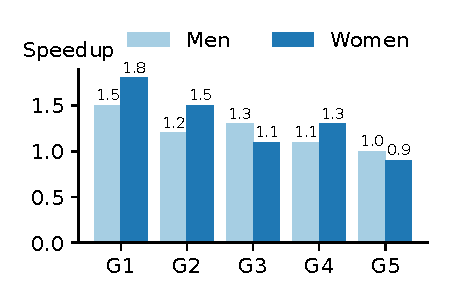
\includegraphics{plots/speedup}
\caption{Improved running speed after 4 weeks of training.
}
\label{fig:speedup}
\end{figure}

\subsubsection{Tables} We optimize our tables for readability by removing as
much clutter as possible, while highlighting the key structure. Markus Püschel
(see doc/paper-writing/guide-tables.pdf) wrote a nice guide on how to make nice
tables. \autoref{tab:simple_table} illustrates this with a simple
table.

\begin{table}
\ra{1.2}
\centering
\begin{tabular}{l l l r}
  \toprule
  \textbf{Animal} & \textbf{Size} & \textbf{Biotope} & \textbf{Age}\\
  \midrule
  Dog & Medium & Ground & 20\\
  Cat & Medium & Ground &20 \\
  Ant & Small & Ground & 30 \\
  Elephant & Large & Ground & 70\\
  Whale & Large & Water & 100\\
  Salmon & Medium & Water & 13 \\
  Eagle & Large & Air & 35 \\
  \bottomrule
\end{tabular}
\vspace{1em}
\caption{A table with heigh lines and emphasized header.}
\label{tab:simple_table}
\end{table}

\subsubsection{Listings} We aim to use minted to create listings as much as
possible, as this allows us to edit code quickly. We use syntax highlighting
to make the parts of the code that matter most stand out. Hence, we keep
most code black, comments gray, and highlight just the MLIR operands that
we care about most.

\begin{listing}[H]
% We cannot put '{' on a line after % in draftonly mode, as the hack we used to
% not include the draft section will interpret the listing as normal
% latex where '%' is a comment and {} need to match, which they will
% not if only one is commented.
\begin{mlir}
// This is a comment
def @foo(%0 : !dialect.type)
{
  %a = dialect.op(%0) : !dialect.type // $\color{black}\circled{a}$
}
\end{mlir}
\caption{A simple MLIR code example with markers. Markers can also be placed in
	captions and refer to labels, e.g. \circled[lst:example]{a}.}
\label{lst:example}
\end{listing}

\begin{listing}[H]
\begin{lean4}
theorem funext {f₁ f₂ : ∀ (x : α), β x}
  (h : ∀ x, f₁ x = f₂ x) : f₁ = f₂ := by
  show extfunApp (Quotient.mk' f₁) = 
       extfunApp (Quotient.mk' f₂)
  apply congrArg
  apply Quotient.sound
  exact h
\end{lean4}
\caption{A simple Lean4 code example, taken from
  \url{https://lean-lang.org/lean4/doc/syntax\_highlight\_in\_latex.html\#example-with-minted}.}
\end{listing}

The syntax highlighting also works for xDSL-like IRs. Notice that different
minted styles can be used for different environments. The xDSL environment uses
the murphy-style in this case, whereas the MLIR version applies the
colorful-style.

\begin{xdsl*}{fontsize=\scriptsize}
func.func() [sym_name = "main", function_type = !fun<[
              !iterators.columnar_batch<!tuple<[!i64]>>
                 ], []>] {
  ^bb0(%0 : !iterators.columnar_batch<!tuple<[!i64]>>):
    %t : !iterators.stream<!llvm.struct<[!i64]>> =
      iterators.scan_columnar_batch(%0 : ...)
    %filtered : !iterators.stream<!llvm.struct<[!i64]>> =
          iterators.filter(%input : …) [predicateRef = @s0]
    iterators.sink(%filtered : !iterators.stream<!tuple<[!i64]>>)
    func.return()
}

func.func() [sym_name = "s0", function_type = !fun<[
    !llvm.struct<[!i64]>], [!i1]>] {
  ^bb0(%struct : !llvm.struct<[!i64]>):
    %id : !i64 = llvm.extractvalue(%struct : ...)
              [position = [0 : !index]]
    %five  : !i64 = arith.constant() [value = 5 : !i64]
    %cmp : !i1 = arith.cmpi(%id : !i64, %five : !i64)
              [predicate = 4 : !i64]
    func.return(%cmp : !i1)
}
\end{xdsl*}

\section{Writing}

A couple of hints with respect to how we write text.

\subsection{Citations}
\label{appendix:citations}

\subsubsection{Do not use numerical citations as nouns}
Especially when working with numerical citations (e.g., [1]) the use of
citations as nouns reduces readability. Hence, we do not use numerical citations
as nouns and instead expand these citations with \texttt{\textbackslash{}citet} to the
authornames.
\\
{\color{pairedTwoDarkBlue}
\textit{[1] showed that .. $\dots$}}\\
$\to$ {\color{pairedFourDarkGreen}\textit{Author et al. [1] showed}}

\subsubsection{Prefer meaningful text over citations as textual content}
While acknowledging authors of work is important, maximizing the amount of technical
content (outside of a historic perspective) typically makes text more direct and
concrete. Hence, we avoid the discussion of who did what in text if the
historic context does not add meaning or empty words can be replaced by an immediate
citation. E.g, in the following the words `introduced in` are not carrying
information and can be dropped.\\
{\color{pairedTwoDarkBlue}
\textit{we extend PreviousIdea introduced in [1] $\dots$ by}}\\
$\to$ {\color{pairedFourDarkGreen}\textit{we extend PreviousIdea [1] by}}


\subsubsection{Managing acronyms automatically}
Managing acronyms manually can lead to situations where the specific term is not properly expanded upon first use or when it is introduced.
The \texttt{acronym} package is useful to avoid such situations and provides full control over acronyms.
The expanded form of an abbreviation should be in lowercase, unless its parts are also capitalized (e.g., United Kingdom for UK).
For example, assume we have defined an acronym with \texttt{\textbackslash{}newacronym\{ir\}\{IR\}\{intermediate representation\}}:
\begin{itemize}
  \item Upon first use of \texttt{\textbackslash{}ac\{ir\}} we get: \ac{ir}.
  \item On the second reference: \ac{ir}.
  \item To force expansion (e.g., for the background section where the term is first described), we use \texttt{\textbackslash{}acf\{ir\}} which gives: \acf{ir}.
  \item To force contraction (e.g., to save space for a figure caption), we use \texttt{\textbackslash{}acs\{ir\}} which gives: \acs{ir}.
  \item To obtain plural form, we use \texttt{\textbackslash{}acp\{ir\}} giving: \acp{ir}.
\end{itemize}

\subsubsection{Adding hyphenation rules}
While \LaTeX\ handles word breaks automatically, and packages like \texttt{microtype} aim to minimize word splitting, there are instances where either new words lack hyphenation rules, or the suggested hyphenation for a word is undesirable.
The \texttt{hyphenat} package allows adding hyphenation rules using the \texttt{\textbackslash{}hyphenation} macro, e.g., \texttt{\textbackslash{}hyphenation\{Alex-Net\}} for AlexNet.

Allowing hyphenation of compound words, we can use \texttt{\textbackslash{}-/} from the \texttt{extdash} package, for example \texttt{high\-/level} can be written as \texttt{high\textbackslash{}-/level}.
Disallowing a line break at the compound word hyphen, we can use \texttt{\textbackslash{}=/}, as \texttt{RISC\textbackslash{}=/V} for \texttt{RISC\=/V}.

\end{draftonly}


\end{document}
